% Figure — The illustration of the ACO undersampler.
% Build (dari manuscript/latex/):
%   pdflatex -output-directory=figures figures/F0b_aco.tex
%   cp figures/F0b_aco.pdf ../F0b_aco.pdf
\documentclass[tikz,border=8pt]{standalone}
\usetikzlibrary{arrows.meta,positioning,decorations.pathreplacing,calc}
\usepackage{amsmath,amsbsy}

\begin{document}
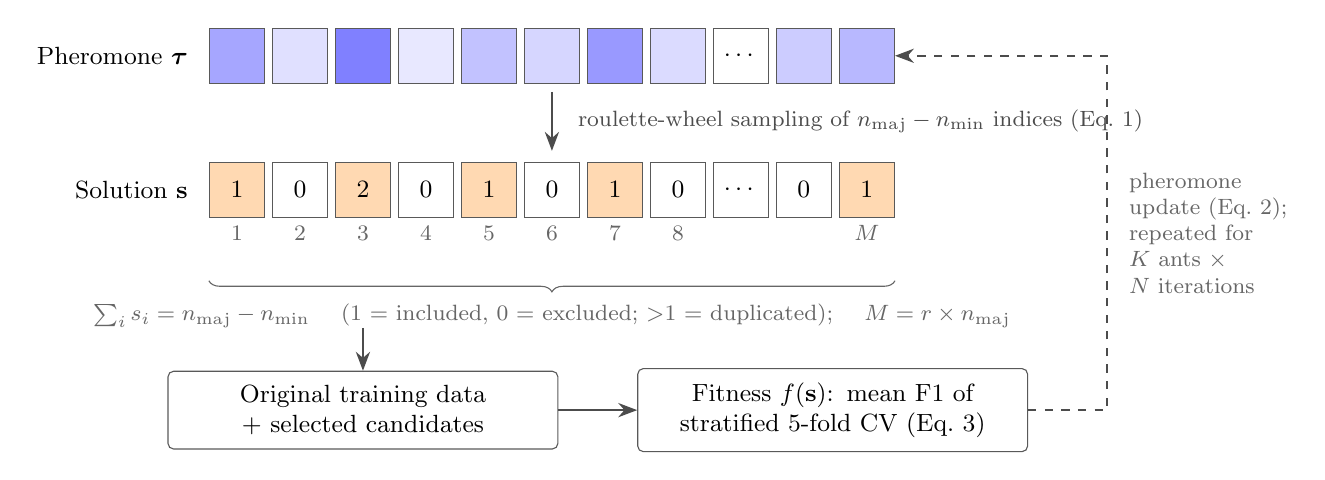
\begin{tikzpicture}[
  font=\small,
  cell/.style={draw=black!65, minimum size=7mm, inner sep=0pt},
  box/.style={draw=black!65, rounded corners=2pt, align=center,
              inner sep=5pt, minimum height=9mm},
  arr/.style={-{Stealth[length=2.4mm]}, thick, black!70},
  dasharr/.style={arr, dashed},
  lab/.style={font=\small, anchor=east},
  note/.style={font=\footnotesize, black!60},
]

\def\dx{8mm}

% ---------- pheromone vector ----------
\foreach [count=\i] \v in {35,12,50,9,24,16,40,14,-1,20,28} {
  \pgfmathsetmacro\x{\i*8}
  \ifnum\v=-1
    \node[cell, fill=white] (tau\i) at (\x mm, 0) {$\cdots$};
  \else
    \node[cell, fill=blue!\v!white] (tau\i) at (\x mm, 0) {};
  \fi
}
\node[lab] at (3mm, 0) {Pheromone $\boldsymbol{\tau}$};

% ---------- sampling arrow ----------
\draw[arr] ($(tau6.south)+(0,-1mm)$) -- ($(tau6.south)+(0,-8.5mm)$)
  node[midway, right=2mm, align=left, font=\footnotesize]
  {roulette-wheel sampling of $n_{\mathrm{maj}}-n_{\min}$ indices
   (Eq.~1)};

% ---------- solution vector ----------
\begin{scope}[yshift=-17mm]
\foreach [count=\i] \v in {1,0,2,0,1,0,1,0,-1,0,1} {
  \pgfmathsetmacro\x{\i*8}
  \ifnum\v=-1
    \node[cell, fill=white] (s\i) at (\x mm, 0) {$\cdots$};
  \else
    \ifnum\v=0
      \node[cell, fill=white] (s\i) at (\x mm, 0) {$0$};
    \else
      \node[cell, fill=orange!30] (s\i) at (\x mm, 0) {$\v$};
    \fi
  \fi
}
\node[lab] at (3mm, 0) {Solution $\mathbf{s}$};
% candidate indices
\foreach [count=\i] \t in {1,2,3,4,5,6,7,8,{},{},{$M$}} {
  \pgfmathsetmacro\x{\i*8}
  \node[note] at (\x mm, -5.5mm) {\t};
}
% constraint brace
\draw[decorate, decoration={brace, amplitude=4pt, mirror}, black!60]
  ($(s1.south west)+(0,-8mm)$) -- ($(s11.south east)+(0,-8mm)$)
  node[midway, below=5pt, note]
  {$\sum_i s_i = n_{\mathrm{maj}} - n_{\min}$
   \quad (1 = included, 0 = excluded; $>$1 = duplicated);
   \quad $M = r \times n_{\mathrm{maj}}$};
\end{scope}

% ---------- evaluation flow ----------
\node[box, text width=46mm] (aug) at (24mm, -45mm)
  {Original training data\\ $+$ selected candidates};
\node[box, text width=46mm, right=10mm of aug] (fit)
  {Fitness $f(\mathbf{s})$: mean F1 of\\ stratified 5-fold CV (Eq.~3)};

\draw[arr] ($(s3.south)+(0,-14mm)$) -- (aug.north);
\draw[arr] (aug) -- (fit);

% ---------- pheromone update feedback ----------
\draw[dasharr] (fit.east) -- ++(10mm,0) |- (tau11.east)
  node[pos=0.25, right=1.5mm, align=left, note]
  {pheromone\\ update (Eq.~2);\\ repeated for\\ $K$ ants $\times$\\ $N$ iterations};

\end{tikzpicture}
\end{document}
